\documentclass{beamer}

\usepackage[utf8]{inputenc}
\usepackage[T1]{fontenc}
\usepackage{listings} % Para snippets de código
\lstset{basicstyle=\tiny\ttfamily, breaklines=true} % Config para código
\usetheme{CambridgeUS}
\usetheme{Dresden}
\usecolortheme{dove}
\setbeamertemplate{navigation symbols}{} % Remove symbols to avoid overflows

% Code listing styling
\definecolor{codegreen}{rgb}{0,0.6,0}
\definecolor{codegray}{rgb}{0.5,0.5,0.5}
\definecolor{codepurple}{rgb}{0.58,0,0.82}
\definecolor{backcolour}{rgb}{0.95,0.95,0.92}

\lstdefinestyle{mystyle}{
    backgroundcolor=\color{backcolour},
    commentstyle=\color{codegreen},
    keywordstyle=\color{magenta},
    numberstyle=\tiny\color{codegray},
    stringstyle=\color{codepurple},
    basicstyle=\ttfamily\tiny,
    xleftmargin=15pt,
    frame=single,
    breakatwhitespace=false,
    breaklines=false,
    captionpos=b,
    keepspaces=true,
    firstnumber=auto,
    numbers=left,
    numbersep=7pt,
    showspaces=false,
    showstringspaces=false,
    showtabs=false,
    tabsize=2,
    extendedchars=true,
    texcl=true,
    inputencoding=utf8
}
\lstset{style=mystyle}

\title[Detecção de Deadlocks]{Detecção de Deadlocks e Violação da Ordem de Aquisição de Travas}
\subtitle{Baseado em DEFINITION.md}
\institute{Universidade Federal do Rio Grande do Norte}
\date{16 de julho de 2025}

\newcommand{\cHeader}{../../src/include/lockdep.h}
\newcommand{\cCore}{../../src/lockdep/lockdep_core.c}
\newcommand{\cInterpose}{../../src/interpose/pthread_interpose.c}

\newcommand{\cDining}{../../tests/t05_dining_philosophers.c}

\usepackage[strings]{underscore}

\begin{document}

\begin{frame}
  \titlepage
\end{frame}

\begin{frame}{Integrantes}
\begin{table}[ht]
\centering
\begin{tabular}{|p{6.5cm}|p{4.5cm}|}
\hline
\textbf{Nome} & \textbf{E-mail} \\
\hline

\textbf{Corpo docente} \\

\hline
Samuel Xavier de Souza &
samuel.xavier@ufrn.br \\

\hline
Wedson Torres de Almeida Filho &
wedson.almeida@dca.ufrn.br \\
\hline

\textbf{Corpo discente} \\

\hline
Vinicius de Lima Duarte Sampaio &
vinicius.lima.115@ufrn.edu.br \\

\hline
Emanuel Rawa Gurgel de Araujo Freitas &
emanuelrawa@gmail.com \\

\hline
Arthur Jose Arruda Skeete &
arthurjoskeete@gmail.com \\

\hline
Yuri Maximiliano Brasileiro Santos &
yurimax322@gmail.com \\

\hline
José Henrique Targino Dias Góis &
ze.gois.00@gmail.com \\

\hline
\end{tabular}
\end{table}
\end{frame}

\begin{frame}{Sumário}
  \tableofcontents
\end{frame}

\section{Introdução e Objetivo}
\begin{frame}{Objetivo}
O objetivo deste projeto é estender uma implementação
didática de mutexes feita em sala, adicionando mecanismos
de detecção de deadlocks e/ou verificação da ordem de
aquisição de travas, inspirando-se em abordagens reais
como o lockdep do Linux.
\end{frame}

\begin{frame}{Descrição}
Mutexes garantem exclusão mútua em regiões críticas, mas
quando múltiplas threads acessam múltiplos mutexes
simultaneamente, podem surgir situações de deadlock —
geralmente causadas por espera circular entre threads.

Este projeto propõe duas abordagens complementares:

\item 1. Detecção de deadlocks via grafo de espera:
\begin{itemize}
    \item Monitorar quais threads possuem e quais esperam por cada mutex.
    \item Construir dinamicamente um grafo de espera por recursos.
    \item Detectar ciclos no grafo, sinalizando um deadlock real.
\end{itemize}

\item 2. Detecção de violação da ordem de aquisição de travas (estilo lockdep):
\begin{itemize}
    \item Manter o histórico da ordem em que mutexes são adquiridos por cada thread.
    \item Detectar quando uma thread tenta adquirir mutexes em uma ordem incompatível com a previamente observada, antes que o deadlock ocorra.
    \item Exibir alertas sobre inversões de ordem (e.g., thread A adquire A → B, e thread B tenta B → A).
\end{itemize}
\end{frame}

\section{Teóricos}
\begin{frame}{Conceitos Chave}
  \begin{itemize}
    \item Deadlock: Espera circular (condições de Coffman).
    \item Grafo de Espera: Nodes=threads/resources; ciclo=deadlock real (DFS).
    \item Lockdep-Style: Grafo dependências (nodes=locks, edges=ordem); ciclo=potencial inversão.
  \end{itemize}
\end{frame}

\begin{frame}{ELF Header Information}
\begin{tabular}{l l}
\hline
\textbf{Field} & \textbf{Value} \\
\hline
Magic & 7f 45 4c 46 02 01 01 00 00 00 00 00 00 00 00 00 \\
Class & ELF64 \\
Data & 2's complement, little endian \\
Version & 1 (current) \\
OS/ABI & UNIX - System V \\
ABI Version & 0 \\
Type & DYN (Position-Independent Executable file) \\
Machine & Advanced Micro Devices X86-64 \\
Version & 0x1 \\
Entry point address & 0x1110 \\
\hline
\end{tabular}
\end{frame}

\begin{frame}{ELF Program Headers}
\small
ELF file type is DYN (Position-Independent Executable file)\\
Entry point 0x1110\\
There are 14 program headers, starting offset 64 (bytes into file)
\vspace{3em}
\scriptsize
\begin{tabular}{l l l l 1 1 1 1}
\hline
\textbf{Type} & \textbf{Offset} & \textbf{VirtAddr} & \textbf{PhysAddr} & \textbf{FileSiz} & \textbf{MemSiz} & \textbf{Flags} & \textbf{Align} \\
\hline
PHDR & 0x0040 & 0x0040 & 0x0040 & 0x0310 & 0x0310 & R & 0x8 \\
INTERP$^*$ & 0x0394 & 0x0394 & 0x0394 & 0x001c & 0x001c & R & 0x1 \\
LOAD & 0x0000 & 0x0000 & 0x0000 & 0x0998 & 0x0998 & R & 0x1000 \\
LOAD & 0x1000 & 0x1000 & 0x1000 & 0x0739 & 0x0739 & R E & 0x1000 \\
LOAD & 0x2000 & 0x2000 & 0x2000 & 0x0378 & 0x0378 & R & 0x1000 \\
LOAD & 0x2dc8 & 0x3dc8 & 0x3dc8 & 0x02b8 & 0x03e0 & RW & 0x1000 \\
DYNAMIC & 0x2dd8 & 0x3dd8 & 0x3dd8 & 0x01e0 & 0x01e0 & RW & 0x8 \\
NOTE & 0x0350 & 0x0350 & 0x0350 & 0x0020 & 0x0020 & R & 0x8 \\
\hline
\end{tabular}
$^*$\ [Requesting program interpreter: /lib64/ld-linux-x86-64.so.2]
\end{frame}

\begin{frame}
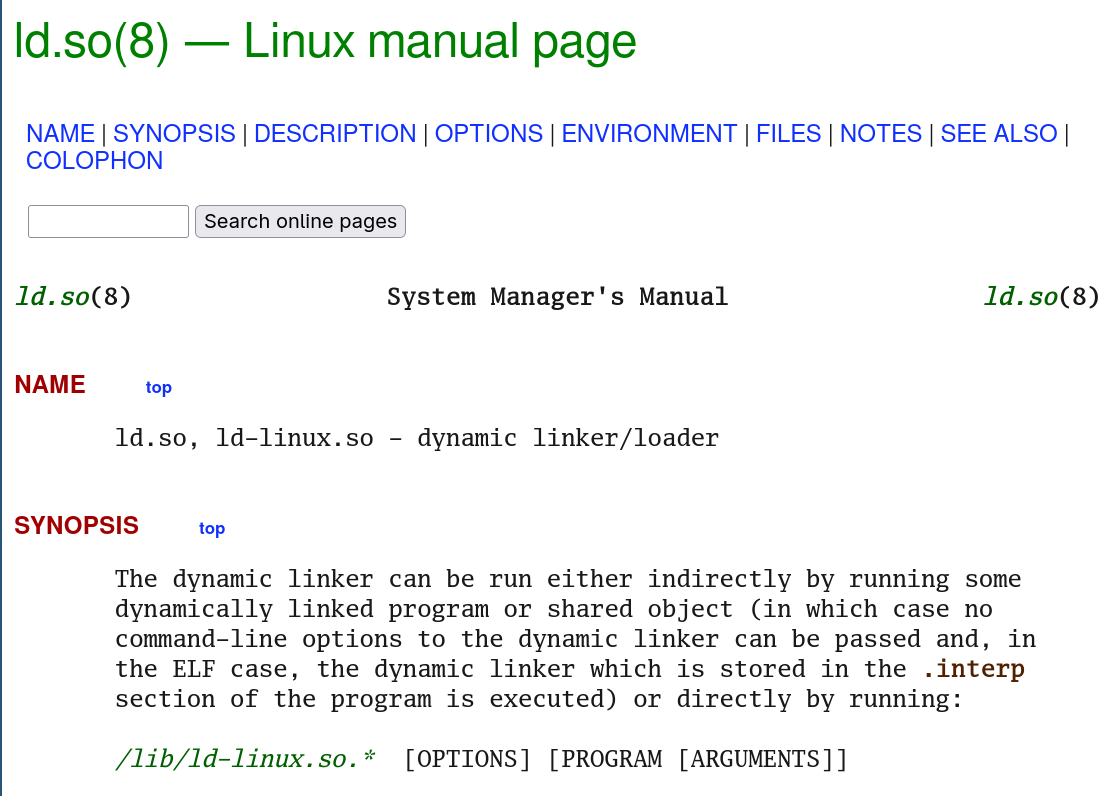
\includegraphics[width=0.9\linewidth]{./ld_linux.png}
\end{frame}

\begin{frame}
\begin{itemize}
\item LD_PRELOAD \\
    A list of additional, user-specified, ELF shared objects to
    be loaded before all others.  This feature can be used to
    selectively override functions in other shared objects.
\end{itemize}
\end{frame}

\section{Implementação por Arquivo}

\begin{frame}{pthread_interpose.c: Hooking Pthread}
  \begin{itemize}
  \item Recebe endereço dos símbolos dinâmicos a serem ligados em tempo de execução;
  \end{itemize}
  \lstinputlisting[language=C, firstnumber=9, firstline=9, lastline=25]{\cInterpose} % Trecho chave
\end{frame}

\begin{frame}{pthread_interpose.c: Hooking Pthread}
  \begin{itemize}
  \item Envelope das funções reais por funções de interposição.
  \end{itemize}
  \lstinputlisting[language=C, firstnumber=37, firstline=37, lastline=49]{\cInterpose} % Trecho chave
\end{frame}

\begin{frame}{pthread_interpose.c: Hooking Pthread}
  \begin{itemize}
  \item Envelope das funções reais por funções de interposição.
  \end{itemize}
  \lstinputlisting[language=C, firstnumber=51, firstline=51, lastline=65]{\cInterpose} % Trecho chave
\end{frame}

\begin{frame}{pthread_interpose.c: Hooking Pthread}
  \begin{itemize}
  \item Envelope das funções reais por funções de interposição.
  \end{itemize}
  \lstinputlisting[language=C, firstnumber=67, firstline=67, lastline=77]{\cInterpose} % Trecho chave
\end{frame}

\begin{frame}{lockdep.h: Estruturas de Dados}
  \begin{itemize}
    \item lock_node_t: Grafo (children) + lista (next); dono (current_held_lock).
    \item adjacency_locks_t: Edges para dependências.
    \item held_lock_t: Pilha de holds com trace e timestamp.
    \item thread_context_t: Contexto thread com pilha held.
  \end{itemize}
\end{frame}

\begin{frame}{lockdep.h: Estruturas de Dados}
    \begin{itemize}
        \item lock_node_t: Grafo (children) + lista (next); dono (current_held_lock).
    \end{itemize}
    \lstinputlisting[language=C, firstnumber=30, firstline=30, lastline=37]{\cHeader}
    \begin{itemize}
        \item adjacency_locks_t: Edges para dependências.
    \end{itemize}
    \lstinputlisting[language=C, firstnumber=40, firstline=40, lastline=43]{\cHeader}
\end{frame}

\begin{frame}{lockdep.h: Estruturas de Dados}
  \begin{itemize}
    \item held_lock_t: Pilha de holds com trace e timestamp.
  \end{itemize}
  \lstinputlisting[language=C, firstnumber=46, firstline=46, lastline=53]{\cHeader}
  \begin{itemize}
    \item thread_context_t: Contexto thread com pilha held.
  \end{itemize}
  \lstinputlisting[language=C, firstnumber=56, firstline=56, lastline=62]{\cHeader}
\end{frame}

\begin{frame}{lockdep_core.c: Lógica Central}
  \begin{itemize}
    \item lockdep_init: Inicializa
    \item lockdep_acquire_lock: Registra, adiciona dep, checa ciclo (DFS).
    \item lockdep_release_lock: Libera, remove
  \end{itemize}
\end{frame}

\begin{frame}{lockdep_core.c: Lógica Central}
  \begin{itemize}
    \item lockdep_init: Inicializa
  \end{itemize}
  \lstinputlisting[language=C, firstnumber=372, firstline=372, lastline=379]{\cCore}
\end{frame}

\begin{frame}{lockdep_core.c: Lógica Central}
  \begin{itemize}
    \item lockdep_acquire_lock: Registra, adiciona dep, checa ciclo (DFS).
  \end{itemize}
  \lstinputlisting[language=C, firstnumber=381, firstline=381, lastline=395]{\cCore}
\end{frame}

\begin{frame}{lockdep_core.c: Lógica Central}
  \begin{itemize}
    \item lockdep_release_lock: Libera, remove
  \end{itemize}
  \lstinputlisting[language=C, firstnumber=397, firstline=397, lastline=404]{\cCore}
\end{frame}

\begin{frame}{lockdep_core.c: Lógica Central}
  \begin{itemize}
    \item lockdep_acquire_lock: Registra, adiciona dep, checa ciclo (DFS).
  \end{itemize}
  \lstinputlisting[language=C, firstnumber=381, firstline=381, lastline=395]{\cCore}
\end{frame}

\begin{frame}{lockdep_core.c: Lógica Central}
  \begin{itemize}
    \item lockdep_acquire_lock: find thread context
  \end{itemize}
  \lstinputlisting[language=C, firstnumber=145, firstline=145, lastline=153]{\cCore}
\end{frame}

\begin{frame}{lockdep_core.c: Lógica Central}
  \begin{itemize}
    \item lockdep_acquire_lock: find or register lock
  \end{itemize}
  \lstinputlisting[language=C, firstnumber=125, firstline=125, lastline=143]{\cCore}
\end{frame}

\begin{frame}{lockdep_core.c: Lógica Central}
  \begin{itemize}
    \item lockdep_acquire_lock: add lock to thread context
  \end{itemize}
  \lstinputlisting[language=C, firstnumber=155, firstline=155, lastline=157, breaklines=true]{\cCore}
  \lstinputlisting[language=C, firstnumber=169, firstline=169, lastline=169]{\cCore}
  \lstinputlisting[language=C, firstnumber=188, firstline=188, lastline=191]{\cCore}
\end{frame}

\begin{frame}{lockdep_core.c: Lógica Central}
  \begin{itemize}
    \item lockdep_acquire_lock: add lock to thread context
  \end{itemize}
  \lstinputlisting[language=C, breaklines=true, firstnumber=158, firstline=158, lastline=167]{\cCore}
\end{frame}

\begin{frame}{lockdep_core.c: Lógica Central}
  \begin{itemize}
    \item lockdep_acquire_lock: add lock to thread context
  \end{itemize}
  \lstinputlisting[language=C, firstnumber=155, firstline=155, lastline=157, breaklines=true]{\cCore}
  \lstinputlisting[language=C, firstnumber=169, firstline=169, lastline=169]{\cCore}
  \lstinputlisting[language=C, firstnumber=188, firstline=188, lastline=191]{\cCore}
\end{frame}

\begin{frame}{lockdep_core.c: Lógica Central}
  \begin{itemize}
    \item lockdep_acquire_lock: add lock to thread context
  \end{itemize}
  \lstinputlisting[language=C, breaklines=true, firstnumber=170, firstline=170, lastline=187]{\cCore}
\end{frame}

\begin{frame}{lockdep_core.c: Lógica Central}
  \begin{itemize}
    \item lockdep_acquire_lock: add dependency to graph
  \end{itemize}
  \lstinputlisting[language=C, firstnumber=212, firstline=212, lastline=232]{\cCore}
\end{frame}

\begin{frame}{lockdep_core.c: has deadlock?}
  \lstinputlisting[language=C, firstnumber=338, firstline=338, lastline=364]{\cCore}
\end{frame}

\section{Exemplo de Execução}

% ADICIONAR AQUI!!!

\section{Conclusão e Extensões}
\begin{frame}{Conclusão}
  \begin{itemize}
    \item Atende lockdep-style; demonstra grafos em concurrency.
    \item Limitações: O(n) lookups (add hash); sem fila wait full.
    \item Impacto: Educacional; usa IA para análise.
  \end{itemize}
\end{frame}

\begin{frame}{Extensões Futuras}
  \begin{itemize}
    \item Implementar grafo espera: Add fila waiters, DFS thread-lock.
    \item Suporte a outros sync (condvars, RW locks).
    \item Otimizações: Hash para lookups; integração gdb/valgrind.
  \end{itemize}
\end{frame}

\begin{frame}{Perguntas?}
  \centering
  \Huge Obrigado! Dúvidas?
\end{frame}

\end{document}
